\documentclass[12pt,letterpaper]{article}

\usepackage[utf8]{inputenc}
\usepackage[T1]{fontenc}
\usepackage{amsmath}
\usepackage{amsfonts}
\usepackage{amssymb}
\usepackage{amsthm}
\usepackage[left=2cm,right=2cm,top=2cm,bottom=2cm,headheight=22pt]{geometry}
\usepackage{fancyhdr}
\usepackage{setspace}
\usepackage{lastpage}
\usepackage{graphicx}
\usepackage{caption}
\usepackage{subcaption}
\usepackage{paralist}
\usepackage{url}

\theoremstyle{definition}
\newtheorem{question}{Question}
\newtheorem{example}{Example}
\newtheorem{exercise}[question]{Exercise}
\newtheorem*{challenge}{Challenge}
\newtheorem*{theorem}{Theorem}
\newtheorem*{definition}{Definition}

\begin{document}

%Paramètres de mise en forme des paragraphes selon les normes françaises
\setlength{\parskip}{1ex plus 0.5ex minus 0.2ex}
\setlength{\parindent}{0pt}

%Paramètres relatifs aux en-têtes et pieds de page.
\pagestyle{fancy}
\lhead{Theron J Hitchman}
\chead{\Large Reading and Guided Practice \#12}
\rhead{Fall 2013}
\lfoot{\emph{Math and Decision Making}}
\cfoot{}
\rfoot{\emph{\thepage\ of \pageref{LastPage}}}

\section*{Introduction}
This reading is about a numerical invariant for knots, called the \emph{unknotting number}.

\section*{Goals}
At the end of this assignment, a student should be able to:
\begin{compactitem}
\item Describe a method for changing crossings that will unknot any knot, and explain why it works.
\item Compute the unknotting number for knots with a small number of crossings.
\item Explain why computing unknotting number is challenging in general.
\end{compactitem}
A student might also be able to:
\begin{compactitem}
\item Solve an open problem about unknotting numbers.
\end{compactitem}

\section*{Reading and Questions for 25 September}

\begin{theorem}
Let $K$ be a knot.
By changing some subset of the crossings, it is possible to change $K$ into the unknot.
\end{theorem}

Here is a recipe for doing this.
Pick a point $P$ on the knot, and some direction of travel away from $P$.
As you ``walk along the knot,'' each time you reach a new crossing and are travelling on the understrand through that crossing, change the roles of understrand and overstrand.
If you reach a crossing you have been through before, or if you reach a new crossing first by taking an overstrand, leave that crossing alone.
The process stops when you reach $P$ again.

Here is an example of the process in action with the knot $8_{20}$.

\begin{figure}[h]
    \centering
    \begin{subfigure}{.3\textwidth}
        \centering
        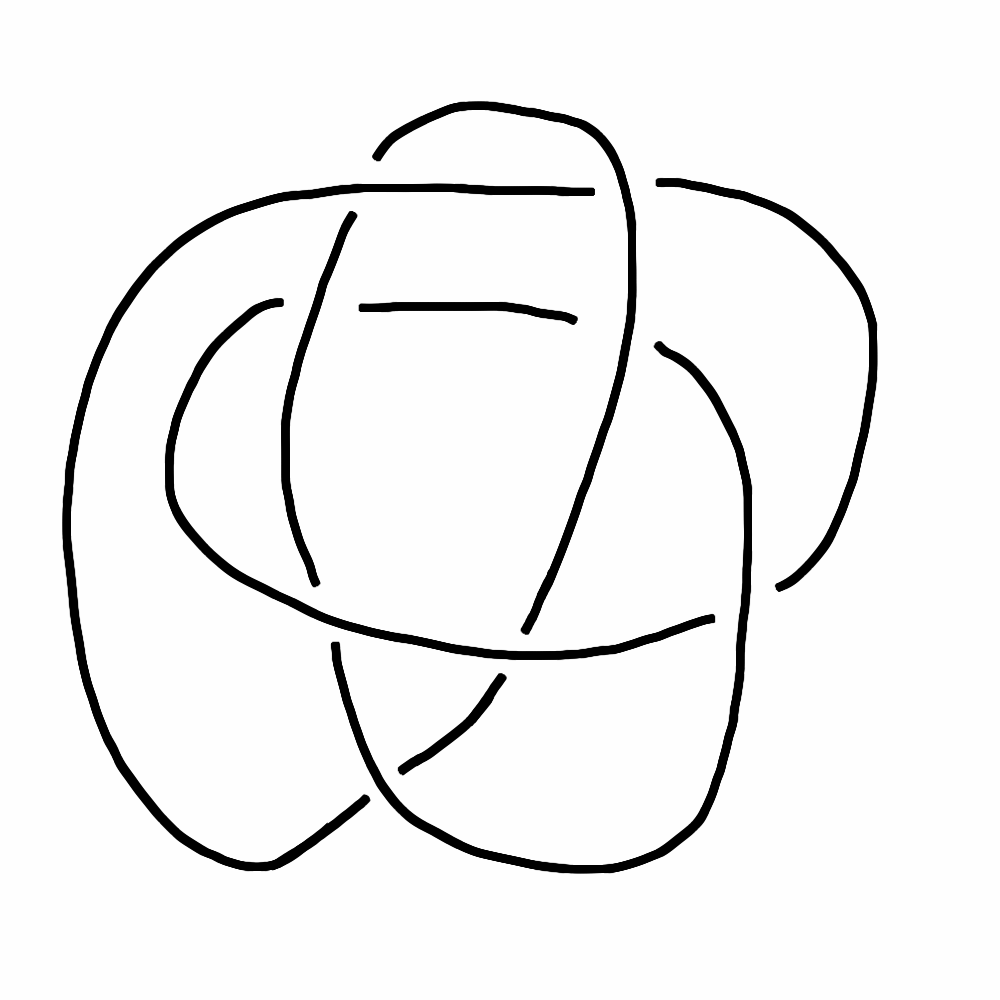
\includegraphics[width=\textwidth]{rgp12pics/8-20.png}
        \caption{The knot $8_{20}$.}
    \end{subfigure}
    \begin{subfigure}{.3\textwidth}
        \centering
        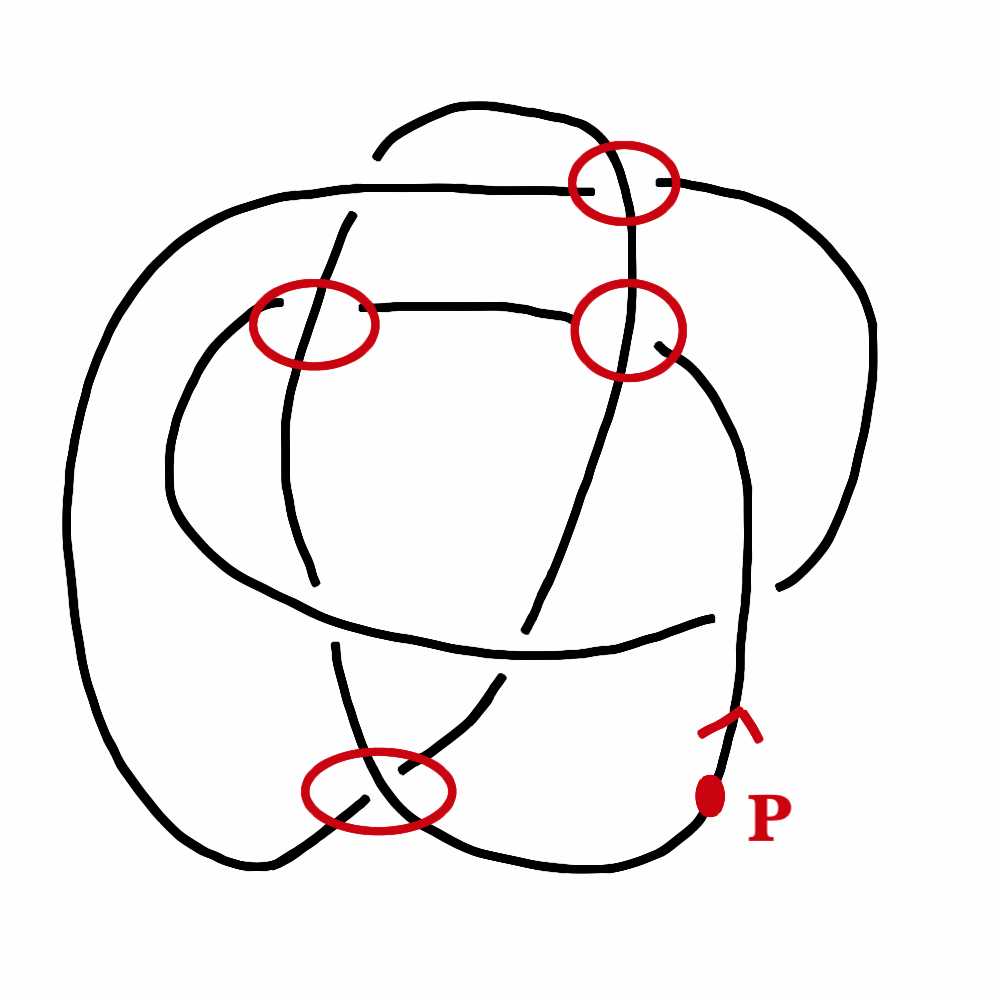
\includegraphics[width=\textwidth]{rgp12pics/8-20-changes.png}
        \caption{The knot $8_{20}$ with spots for changes labeled.}
    \end{subfigure}
    \begin{subfigure}{.3\textwidth}
        \centering
        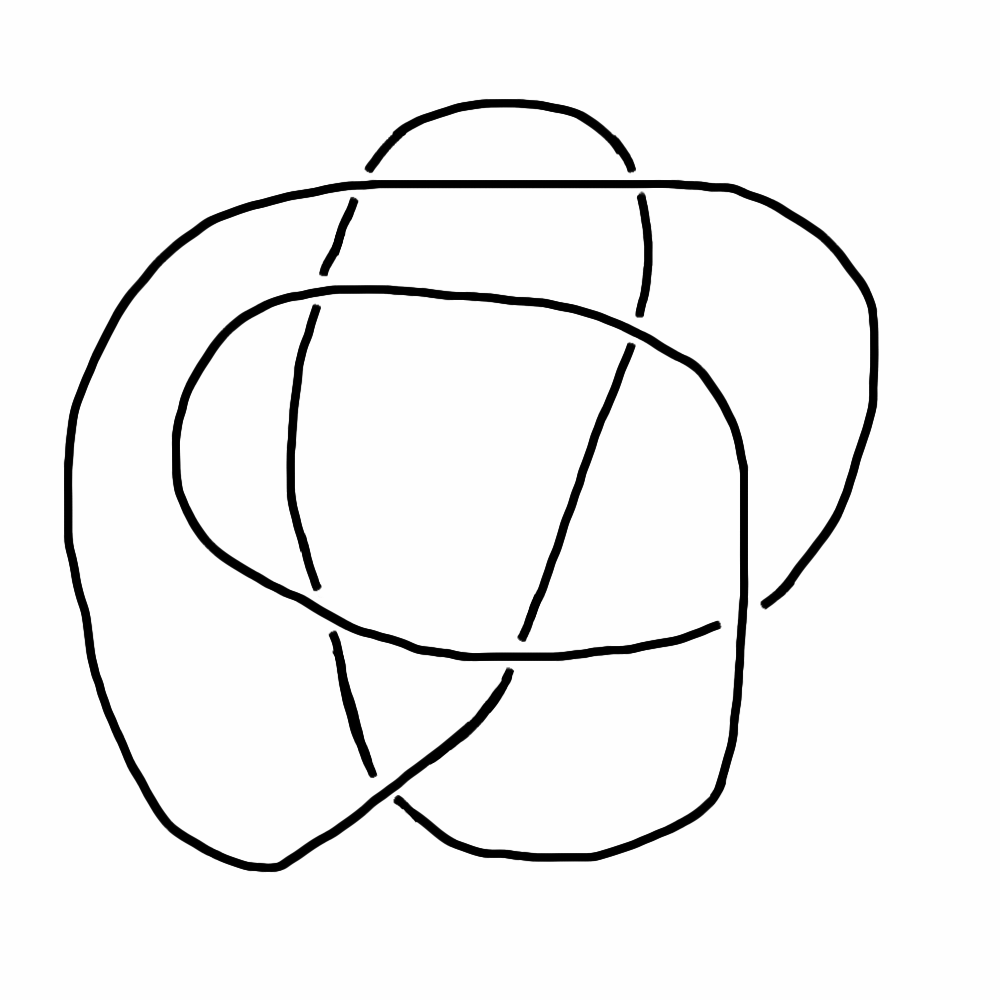
\includegraphics[width=\textwidth]{rgp12pics/8-20-unknot.png}
        \caption{After changes---the unknot.}
    \end{subfigure}
    \caption{Changing crossings to unknot a knot.}
\end{figure}

\clearpage

\begin{exercise}
Try the process yourself on the trefoil knot.
\end{exercise}

\begin{figure}[h]
    \centering
    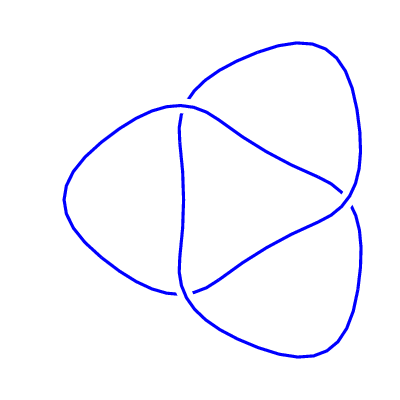
\includegraphics[width=.3\textwidth]{rgp12pics/3_1.png}
    \caption{The trefoil knot}
\end{figure}

This process is enough to prove the theorem, because it \emph{always} works.
That is, after following this process, you will always end up with the unknot.

\begin{challenge}
Why does that process always work?
\end{challenge}


\section*{The Unknotting Number of a Knot}

The theorem we just explored allows us to make a definition of a new invariant. This invariant will be a number, much like linking number for links, but it will only work for knots.

\begin{definition}
Let $K$ be a knot.
The \emph{unknotting number} of $K$, denoted $u(K)$, is the smallest number of crossing changes needed to get the unknot, where we allow consideration of \underline{any} projection of the knot.
\end{definition}

The unknotting number is notoriously hard to compute when the number of crossings gets too big. 
And by ``too big," we mean bigger than about nine or ten. 
The trouble is that you have to find some way to be sure that there is no other projection of your knot that makes the crossing changes more convenient! 
There are lots of possibilities.

Of course, even for small knots things can be challenging and time-consuming. 
It may be that a small number of changes will work, but you still do not know \emph{which} changes are the important ones.
One usually has to try all of the crossings in combinations.
If one is unsure about how to proceed with a given knot, it is best to stay organized and work carefully through all of the possible single crossing changes, then all of the possible pairs of changes, then all of the possible triples of changes, \dots until one has found something which transforms the knot into the unknot. 
If at the same time you have reasons why none of the the other crossing changes will work out, then you have computed the unknotting number.

\clearpage

\begin{exercise}
Below is a table of some knots with small numbers of crossings.
First, find a way to change the indicated number of crossings to make the knot into the unknot.
Second, find a way to argue why the unknotting number cannot be any smaller than that number.
Both halves gives a complete argument for why the unknotting number is as listed.
\end{exercise}
\begin{center}
\begin{tabular}{lr}
knot $K$ & unknotting number $u(K)$ \\
\hline
the unknot & $0$ \\
the trefoil & $1$ \\
the figure eight knot & $1$ \\
the knot $5_2$ (see below) & $1$
\end{tabular}
\end{center}

\begin{figure}[h]
    \centering
    \begin{subfigure}{.4\textwidth}
        \centering
        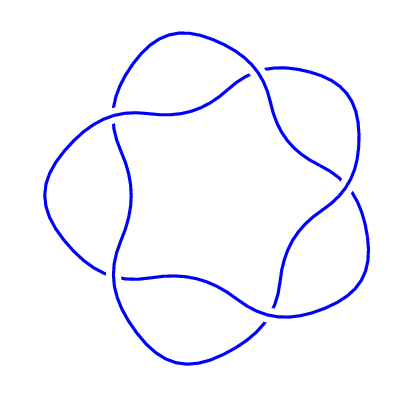
\includegraphics[width=\textwidth]{rgp12pics/5_1.png}
        \caption{The knot $5_1$}
    \end{subfigure}
    \hspace{1in}
    \begin{subfigure}{.4\textwidth}
        \centering
        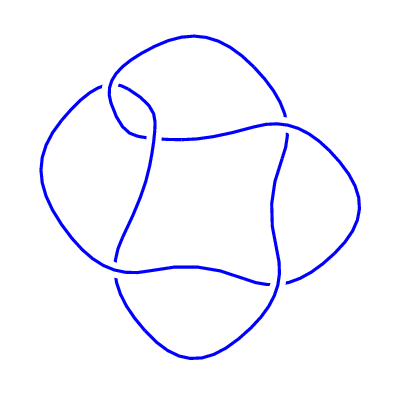
\includegraphics[width=\textwidth]{rgp12pics/5_2.png}
        \caption{The knot $5_2$}
    \end{subfigure}
    \caption{The prime knots with $5$ crossings.}
\end{figure}

\begin{exercise}
Show that there is a pair of crossing changes which transforms the knot $5_1$ into the unknot.
This proves that $u(5_1) \leq 2$.
\end{exercise}

\begin{exercise}
Explain why this is not enough to show that $u(5_1) = 2$.
\end{exercise}

In fact, the unknotting number of $5_1$ is equal to $2$. This does have a rigorous proof, but we'll not explore it for lack of time.

\subsection*{Computing Unknotting numbers is \emph{hard}.}

To show off how challenging the computation of unknotting numbers are, here are two knots for which the best known information is a range of values for the unknotting number. 
The exact values of these invariants are open problems. 
If you figure them out, let me know and I'll help you write a paper and get it published in a mathematical journal. 
(It would be a big deal.)
Another reason for writing these down is to demonstrate that mathematics is an active and growing field. Knot theory is an area of current research, and there are many simple-sounding questions still unresolved.

\begin{example}
The knot $10_{11}$ is known to have unknotting number of $2$ or $3$.
It is not known which is the correct value.
\end{example}

\begin{example}
The knot $11a_{354}$ has unknotting number of $2$, $3$ or $4$.
It is not known which is the correct value.
(By the way, this notation $11a_{354}$ means it is entry number 354 on the standard list of prime, alternating knots with eleven crossings.)
\end{example}

\begin{figure}[h!]
    \centering
    \begin{subfigure}{.4\textwidth}
        \centering
        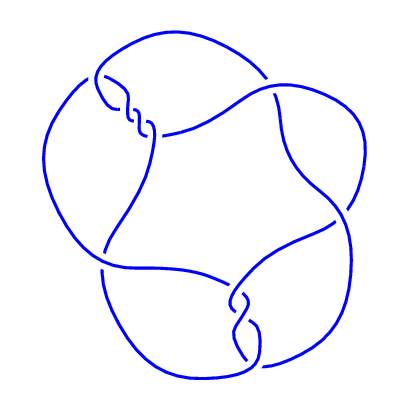
\includegraphics[width=\textwidth]{rgp12pics/10_11.png}
        \caption{The knot $10_{11}$.}
    \end{subfigure}
    \hspace{1cm}
    \begin{subfigure}{.4\textwidth}
        \centering
        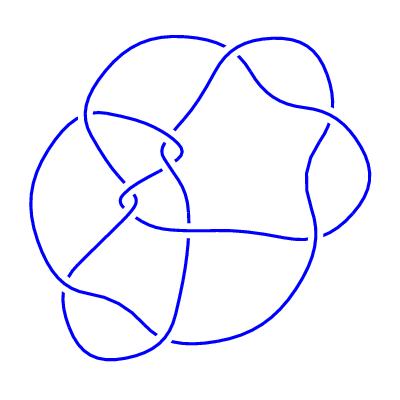
\includegraphics[width=\textwidth]{rgp12pics/11a_354.png}
        \caption{The knot $11a_{354}$.}
    \end{subfigure}
    \caption{Two knots with unknown unknotting numbers.}
\end{figure}

\begin{challenge}
Figure out the exact unknotting numbers for these two knots.
\end{challenge}

As if that wasn't hard enough, things are worse.
There is an example of a knot whose simplest projection, the one with the fewest crossings, has exactly ten crossings. 
Here it is, it is the knot $10_8$
\begin{figure}[h!]
    \centering
    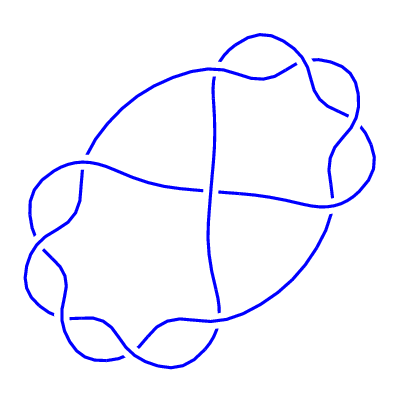
\includegraphics[width=.3\textwidth]{rgp12pics/10_8.png}
    \caption{The standard projection of $10_8$.}
\end{figure}
Even more, it is known that this is the only projection of the knot with ten crossings, up to planar isotopy and mirror reversal.
In this projection, it takes at least $3$ crossing changes to transform this to the unknot.

But there is another projection of this knot with $14$ crossings, which looks like this:
\begin{figure}[h!]
    \centering
    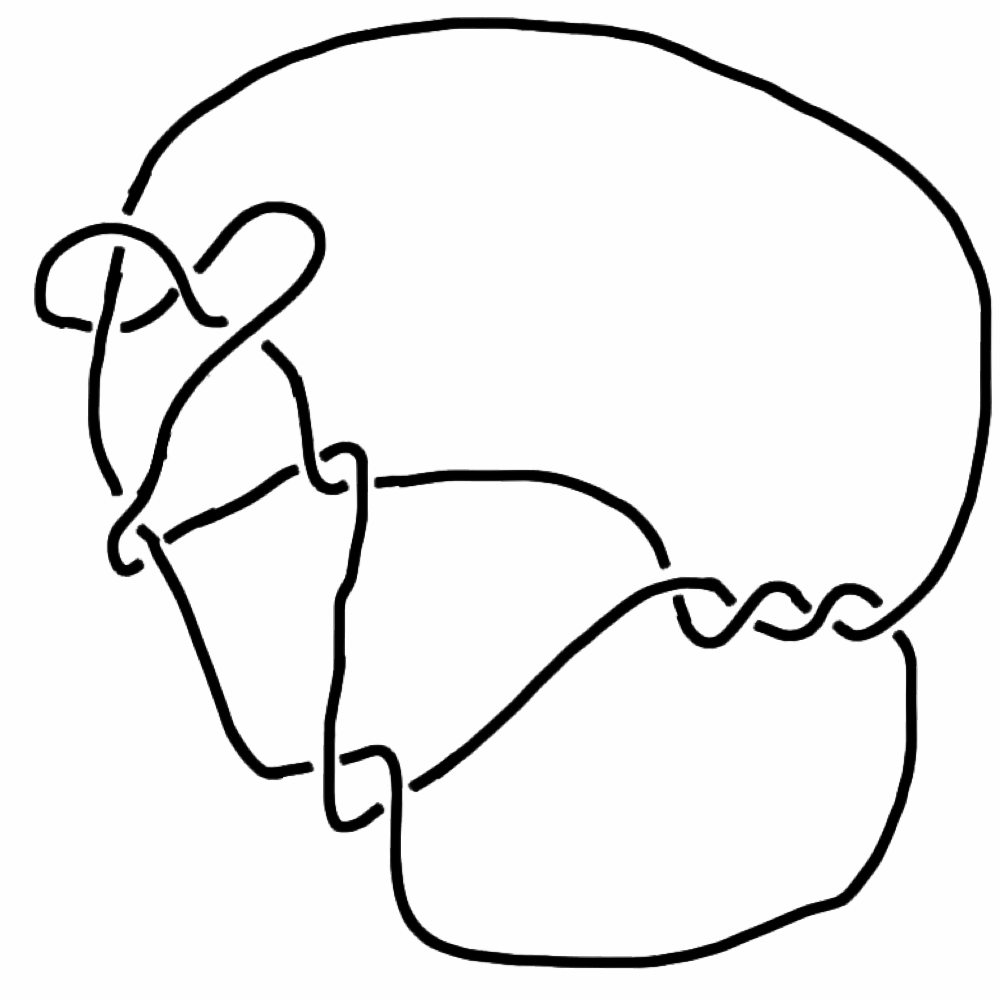
\includegraphics[width=.3\textwidth]{rgp12pics/10-8-14crossings.png}
    \caption{A projection of $10_8$ which has $14$ crossings.}
\end{figure}
In this projection, it is possible to find two crossings which if changed will transform this into the unknot.

\begin{exercise}
Find a set of three crossing changes which turn the standard projection of $10_8$ into the unknot.
Find a set of two crossing changes which turns the alternate projection of $10_8$ into the unknot.
\end{exercise}

The uptake is that the most convenient way to unknot a knot may involve making it more complicated first!
Oh, no!

\subsection*{Conclusion}
This ends our journey into the basics of knot theory.
We have only scratched the surface of what is known, but I think this gives a flavor of the subject. 
I hope you have enjoyed it and found it challenging.
Even more, I hope it makes you re-evaluate what the word ``mathematics'' means.
It is a much larger subject than most people know.

\begin{thebibliography}{9}


\bibitem{Adams}
    C.~Adams,
    \emph{The Knot Book: An elementary introduction to the mathematical theory of knots},
    W.~H.~Freeman Co., New York 1994.

\bibitem{ArtOfMath:knots}
	Philip K. Hotchkiss, with Volker Ecke, Julian F. Fleron, and Christine von~Renesse,
	\emph{Knot Theory},
	available online from \url{http://www.artofmathematics.org/},
	accessed August 15, 2013.

\bibitem{knotinfo}
	J. C. Cha and C. Livingston,
	KnotInfo: Table of Knot Invariants,
	\url{http://www.indiana.edu/~knotinfo},
	accessed: September 6, 2013.


\end{thebibliography}

\end{document}
%sagemathcloud={"zoom_width":100}